\documentclass[a4paper,11pt]{article}

\newcommand{\authorinfo}{Paul Bienkowski, Konstantin Kobs}
\newcommand{\titleinfo}{Robotics Assignment \#04}

% PREAMBLE ===============================================================

\usepackage[german,ngerman]{babel}
\usepackage[utf8]{inputenc}
\usepackage[T1]{fontenc}
\usepackage[top=1.3in, bottom=1in, left=1.0in, right=0.6in]{geometry}
\usepackage{lmodern}
\usepackage{amssymb}
\usepackage{mathtools}
\usepackage{amsmath}
\usepackage{enumerate}
\usepackage{pgfplots}
\usepackage{breqn}
\usepackage{tikz}
\usepackage{fancyhdr}
\usepackage{multicol}
\usepackage{gensymb}
\allowdisplaybreaks

\usetikzlibrary{calc}
\usetikzlibrary{patterns}

\author{\authorinfo}
\title{\titleinfo}
\date{\today}

\pagestyle{fancy}
\fancyhf{}
\fancyhead[L]{\authorinfo}
\fancyhead[R]{\titleinfo}
\fancyfoot[C]{\thepage}

\begin{document}
\maketitle
\begin {enumerate}
	\item[\textbf{Task 4.1.}]
		To calculate the Jacobian matrix, we need the position of the end effector based on the joint angles. Therefore, we need to determine the homogeneous transformation from the base to the end effector point. We can reuse the general transformation matrix given in assignment 2 task 1, because the manipulator shown there is the same as the one in this task. Only $a_i$ needs to be changed to $l_i$. Then we have
		
		$${^{0}T_3} = \begin{pmatrix}
			C_{1+2+3} & -S_{1+2+3} & 0 & C_{1+2+3}l_3 + C_{1+2}l_2+C_1l_1\\
			S_{1+2+3} & C_{1+2+3} & 0 & S_{1+2+3}l_3 + S_{1+2}l_2 + S_1l_1\\
			0 & 0 & 1 & 0\\
			0 & 0 & 0 & 1
		\end{pmatrix}$$
		
		Because this is a planar manipulator, we just need the x and y coodinates. These are $x = C_{1+2+3} \cdot l_3 + C_{1+2} \cdot l_2 + C_1 \cdot l_1$ and $y = S_{1+2+3} \cdot l_3 + S_{1+2} \cdot l_2 + S_1 \cdot l_1$. The Jacobian matrix has to be a $2 \times 3$ matrix, because we have 2 degrees of freedom in cartesian space and 3 degrees of freedom in joint space. The entries of this matrix are the partial derivatives of x and y.
		
		\begin{align*}
			J &= \begin{pmatrix}
				\frac{\partial x}{\partial \theta_1} & \frac{\partial x}{\partial \theta_2} & \frac{\partial x}{\partial \theta_3} \\[6pt]
				\frac{\partial y}{\partial \theta_1} & \frac{\partial y}{\partial \theta_2} & \frac{\partial y}{\partial \theta_3} \\
			\end{pmatrix}\\
			&= \begin{pmatrix}
				-S_{1+2+3} \cdot l_3 - S_{1+2} \cdot l_2 - S_1 \cdot l_1 & -S_{1+2+3} \cdot l_3 - S_{1+2} \cdot l_2 & -S_{1+2+3} \cdot l_3\\
				C_{1+2+3} \cdot l_3 + C_{1+2} \cdot l_2 + C_1 \cdot l_1 & C_{1+2+3} \cdot l_3 + C_{1+2} \cdot l_2 & C_{1+2+3} \cdot l_3
			\end{pmatrix}\\
		\end{align*}
		
		
	\item[\textbf{Task 4.2.}]
		\begin{enumerate}
			\item[1)] The visualization can be found in the following figure. The grey area that looks like a DVD is the reachable workspace of the arm. The red area depicts the space the second link can reach.
			\begin{center}
				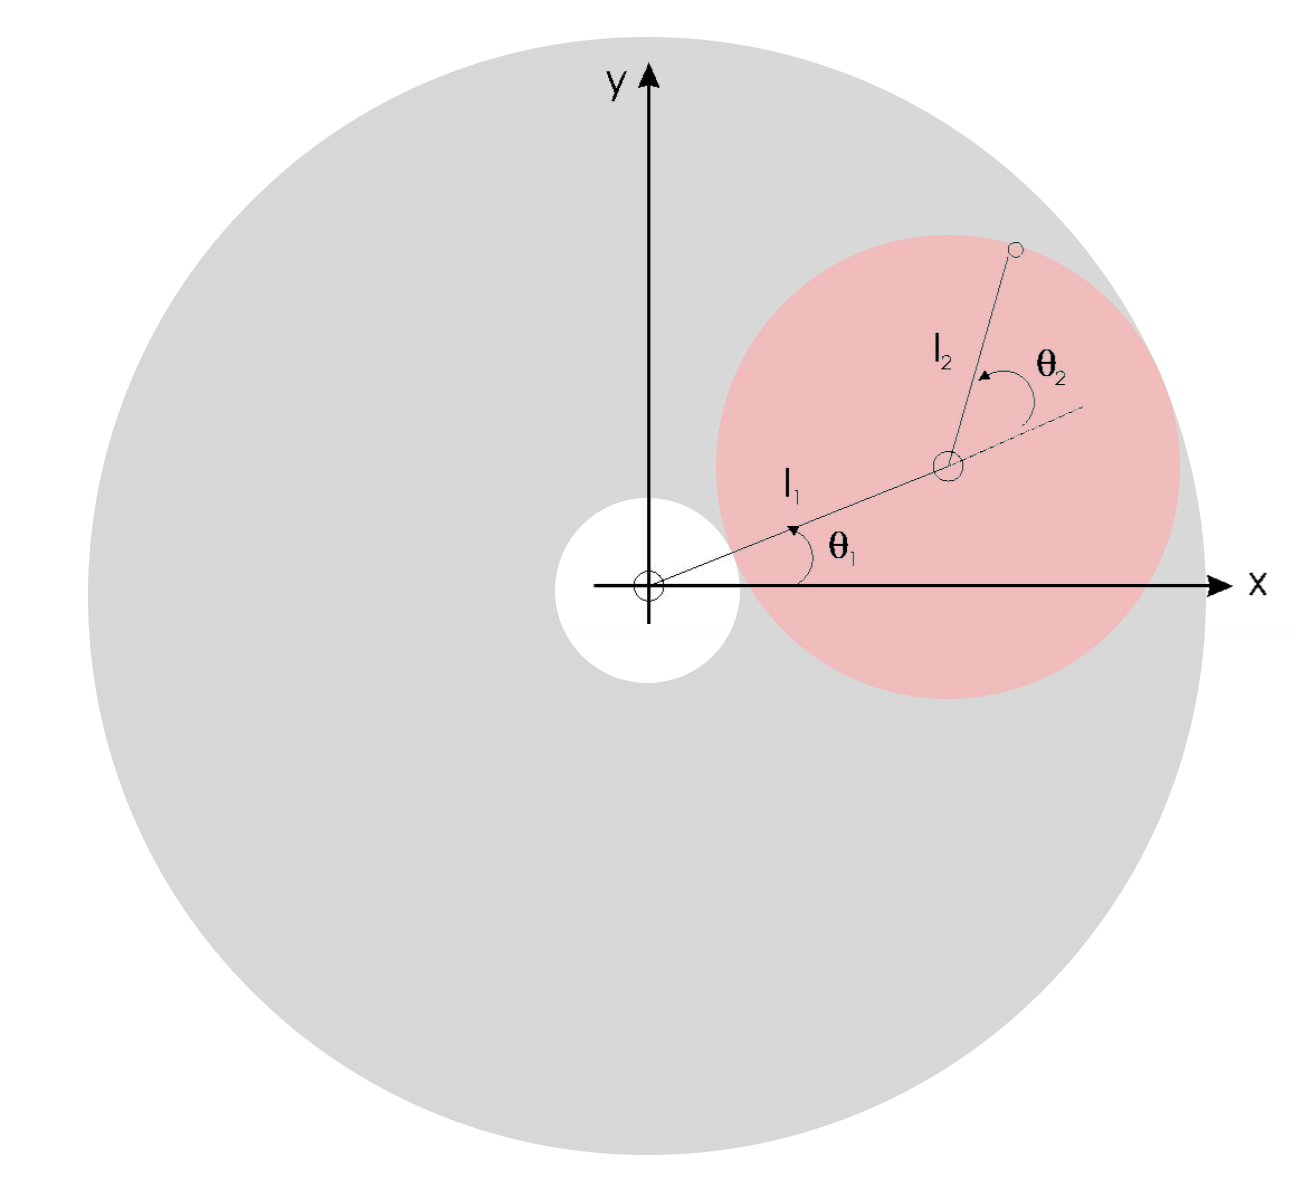
\includegraphics[scale=0.2]{4-2-1.png}
			\end{center}
			
			\item[2)]
				We need the x and y coordinates of the end effector. We can determine these by calculating the transformation matrix and extract the respective entries:
				
				\begin{align*}
					{^0T_1} &= Rot_{z}(\theta_1) \cdot Trans_{x_1}(l_1)\\
					&= \begin{pmatrix}
						C_1 & -S_1 & 0 & l_1 \cdot C_1\\
						S_1 & C_1 & 0 & l_1 \cdot S_1\\
						0 & 0 & 1 & 0\\
						0 & 0 & 0 & 1
					\end{pmatrix}\\
					{^1T_2} &= Rot_{z}(\theta_2) \cdot Trans_{x_2}(l_2)\\
					&= \begin{pmatrix}
						C_2 & -S_2 & 0 & l_2 \cdot C_2\\
						S_2 & C_2 & 0 & l_2 \cdot S_2\\
						0 & 0 & 1 & 0\\
						0 & 0 & 0 & 1
					\end{pmatrix}\\
					{^0T_2} &= {^0T_1} \cdot {^1T_2}\\
					&= \begin{pmatrix}
						C_{1+2} & -S_{1+2} & 0 & C_1 \cdot l_1 + C_{1+2} \cdot l_2 \\
						S_{1+2} & C_{1+2} & 0 & S_1 \cdot l_1 + S_{1+2} \cdot l_2 \\
						0 & 0 & 1 & 0\\
						0 & 0 & 0 & 1
					\end{pmatrix}\\
				\end{align*}
				
				So $x = C_1 \cdot l_1 + C_{1+2} \cdot l_2$ and $y = S_1 \cdot l_1 + S_{1+2} \cdot l_2$.
				
				Given that
				
				$$J = \begin{pmatrix}
					\frac{\partial x}{\partial \theta_1} & \frac{\partial x}{\partial \theta_2} \\[6pt]
					\frac{\partial y}{\partial \theta_1} & \frac{\partial y}{\partial \theta_2}
				\end{pmatrix} \\$$
					
				this leads to
				
				$$J = \begin{pmatrix}
					-S_1 \cdot l_1 - S_{1+2} \cdot l_2 & -S_{1+2} \cdot l_2 \\
					C_1 \cdot l_1 + C_{1+2} \cdot l_2 & C_{1+2} \cdot l_2 \\
				\end{pmatrix} \\$$
				
			\item[3)]
				If the determinant of the Jacobian matrix is zero, then the matrix is not invertible and therefore singular. This is why we need to calculate the determinant of the previously calculated matrix and set it equal to zero:
				
				\begin{align*}
					\det(J) &= 0\\
					&= (-S_1 \cdot l_1 - S_{1+2} \cdot l_2) \cdot (C_{1+2} \cdot l_2) - (-S_{1+2} \cdot l_2) \cdot (C_1 \cdot l_1 + C_{1+2} \cdot l_2)\\
					&= - (S_1 \cdot l_1 \cdot C_{1+2} \cdot l_2) - (S_{1+2} \cdot l_2 \cdot C_{1+2} \cdot l_2) + (S_{1+2} \cdot l_2 \cdot C_1 \cdot l_1) + (S_{1+2} \cdot l_2 \cdot C_{1+2} \cdot l_2) \\
					&= - (S_1 \cdot l_1 \cdot C_{1+2} \cdot l_2) + (S_{1+2} \cdot l_2 \cdot C_1 \cdot l_1) \\
					&= l_1 \cdot l_2 \cdot ( S_{1+2} \cdot C_1 - C_{1+2} \cdot S_1 )\\
					&\overset{\text{sum rule}}{=} l_1 \cdot l_2 \cdot S_{1+2-1}\\
					&= l_1 \cdot l_2 \cdot S_{2} = 0
				\end{align*}
				
				We assume that both lengths $l_1$ and $l_2$ are bigger than zero, therefore $S_2$ has to be zero. That happens, when $\theta_2 = 0\degree$ or $\theta_2 = 180\degree$. So these are the singular configurations of the manipulator.
				
			\item[4)] If $\theta_2$ is zero or 180 degree, the manipulator will be at the edge of its workspace. So the possibility of moving any further than that is not there. The singularity is when the joint velocity becomes infinite to maintain cartesian velocity. That is the case, because we cannot go any further than this.
			
		\end{enumerate}				
		
		
	\item[\textbf{Task 4.3.}]
		\begin{enumerate}
			\item If $\theta_3$ is zero, assuming that the figure shows the default configuration of the robot arm, then the TCP is at the edge of its workspace. Therefore, the manipulator has a singularity at this configuration.
			\item Assuming the length $a_2$ is much longer than the length $d_4$, then the arm can fold back in at $\theta_3 = 180\degree$ and therefore, we have a workspace boundary singularity here as well.
		\end{enumerate}
	
	\item[\textbf{Task 4.4.}]
		We will combine rotations, that we can easily calculate, to get the overall matrix around an arbitrary vector $k$. This will be established by:
		\begin{enumerate}
			\item rotating the vector $k$ about the global z axis to align it with the (x,z) plane (we call this angle $\alpha$).
			\item rotating the vector about the global y axis to align it with the global x axis (we call this angle $\beta$). Now rotating about $k$ is equal to rotating about the global x axis.
			\item rotating about the global x axis/k by $\theta$.
			\item reversing the rotation about the global y axis.
			\item reversing the rotation about the global z axis.
		\end{enumerate}
		
		Because we use Roll-Pitch-Yaw angles, we need to append a new rotation matrix on the left side.	 Finally, we can calculate the resulting matrix with this formula:
		
		$$Rot_{k, \theta} = Rot_{z}(-\alpha) \cdot Rot_{y}(-\beta) \cdot Rot_{x}(\theta) \cdot Rot_{y}(\beta) \cdot Rot_{z}(\alpha)$$
		
		This leads to:
		
		\begin{align*}
			Rot_{k, \theta} &= Rot_{z}(-\alpha) \cdot Rot_{y}(-\beta) \cdot Rot_{x}(\theta) \cdot Rot_{y}(\beta) \cdot Rot_{z}(\alpha)\\
			&= \begin{pmatrix}
				C_{-\alpha} & -S_{-\alpha} & 0 & 0\\
				S_{-\alpha} & C_{-\alpha} & 0 & 0\\
				0 & 0 & 1 & 0\\
				0 & 0 & 0 & 1\\
			\end{pmatrix} \begin{pmatrix}
				C_{-\beta} & 0 & S_{-\beta} & 0\\
				0 & 1 & 0 & 0\\
				-S_{-\beta} & 0 & C_{-\beta} & 0\\
				0 & 0 & 0 & 1\\
			\end{pmatrix} \begin{pmatrix}
				1 & 0 & 0 & 0\\
				0 & C_{\theta} & -S_{\theta} & 0\\
				0 & S_{\theta} & C_{\theta} & 0\\
				0 & 0 & 0 & 1\\
			\end{pmatrix}\\
			&\qquad \begin{pmatrix}
				C_{\beta} & 0 & S_{\beta} & 0\\
				0 & 1 & 0 & 0\\
				-S_{\beta} & 0 & C_{\beta} & 0\\
				0 & 0 & 0 & 1\\
			\end{pmatrix} \begin{pmatrix}
				C_{\alpha} & -S_{\alpha} & 0 & 0\\
				S_{\alpha} & C_{\alpha} & 0 & 0\\
				0 & 0 & 1 & 0\\
				0 & 0 & 0 & 1\\
			\end{pmatrix}\\
	% ERSTE UMFORMUNG
			&= \begin{pmatrix}
				C_{-\alpha}C_{-\beta} & -S_{-\alpha} & C_{-\alpha}S_{-\beta} & 0\\
				S_{-\alpha}C_{-\beta} & C_{-\alpha} & S_{-\alpha}S_{-\beta} & 0\\
				-S_{-\beta} & 0 & C_{-\beta} & 0\\
				0 & 0 & 0 & 1\\
			\end{pmatrix} \begin{pmatrix}
				1 & 0 & 0 & 0\\
				0 & C_{\theta} & -S_{\theta} & 0\\
				0 & S_{\theta} & C_{\theta} & 0\\
				0 & 0 & 0 & 1\\
			\end{pmatrix}\\
			&\qquad \begin{pmatrix}
				C_{\beta} & 0 & S_{\beta} & 0\\
				0 & 1 & 0 & 0\\
				-S_{\beta} & 0 & C_{\beta} & 0\\
				0 & 0 & 0 & 1\\
			\end{pmatrix} \begin{pmatrix}
				C_{\alpha} & -S_{\alpha} & 0 & 0\\
				S_{\alpha} & C_{\alpha} & 0 & 0\\
				0 & 0 & 1 & 0\\
				0 & 0 & 0 & 1\\
			\end{pmatrix}\\
	% ZWEITE UMFORMUNG
			&= \begin{pmatrix}
				C_{-\alpha}C_{-\beta} & -S_{-\alpha} & C_{-\alpha}S_{-\beta} & 0\\
				S_{-\alpha}C_{-\beta} & C_{-\alpha} & S_{-\alpha}S_{-\beta} & 0\\
				-S_{-\beta} & 0 & C_{-\beta} & 0\\
				0 & 0 & 0 & 1\\
			\end{pmatrix} \begin{pmatrix}
				1 & 0 & 0 & 0\\
				0 & C_{\theta} & -S_{\theta} & 0\\
				0 & S_{\theta} & C_{\theta} & 0\\
				0 & 0 & 0 & 1\\
			\end{pmatrix}\\
			&\qquad \begin{pmatrix}
				C_{\beta}C_{\alpha} & -S_{\alpha}C_{\beta} & S_{\beta} & 0\\
				S_{\alpha} & C_{\alpha} & 0 & 0\\
				-S_{\beta}C_{\alpha} & S_{\beta}S_{\alpha} & C_{\beta} & 0\\
				0 & 0 & 0 & 1\\
			\end{pmatrix}\\
	% DRITTE UMFORMUNG
			&= \begin{pmatrix}
				C_{-\alpha}C_{-\beta} & -S_{-\alpha}C_{\theta}+C_{-\alpha}S_{-\beta}S_{\theta} & S_{-\alpha}S_{\theta}+C_{-\alpha}S_{-\beta}C_{\theta} & 0\\
				S_{-\alpha}C_{-\beta} & C_{-\alpha}C_{\theta}+S_{-\alpha}S_{-\beta}S_{\theta} & -S_{\theta}C_{-\alpha}+S_{-\alpha}S_{-\beta}C_{\theta} & 0\\
				-S_{-\beta} & C_{-\beta}S_{\theta} & C_{-\beta}C_{\theta} & 0\\
				0 & 0 & 0 & 1\\
			\end{pmatrix}\\
			&\qquad \begin{pmatrix}
				C_{\beta}C_{\alpha} & -S_{\alpha}C_{\beta} & S_{\beta} & 0\\
				S_{\alpha} & C_{\alpha} & 0 & 0\\
				-S_{\beta}C_{\alpha} & S_{\beta}S_{\alpha} & C_{\beta} & 0\\
				0 & 0 & 0 & 1\\
			\end{pmatrix}\\
	% VIERTE UMFORMUNG
			&= \begin{pmatrix}
				C_{-\alpha}C_{-\beta} & -S_{-\alpha}C_{\theta}+C_{-\alpha}S_{-\beta}S_{\theta} & S_{-\alpha}S_{\theta}+C_{-\alpha}S_{-\beta}C_{\theta} & 0\\
				S_{-\alpha}C_{-\beta} & C_{-\alpha}C_{\theta}+S_{-\alpha}S_{-\beta}S_{\theta} & -S_{\theta}C_{-\alpha}+S_{-\alpha}S_{-\beta}C_{\theta} & 0\\
				-S_{-\beta} & C_{-\beta}S_{\theta} & C_{-\beta}C_{\theta} & 0\\
				0 & 0 & 0 & 1\\
			\end{pmatrix}\\
			&\qquad \begin{pmatrix}
				C_{\beta}C_{\alpha} & -S_{\alpha}C_{\beta} & S_{\beta} & 0\\
				S_{\alpha} & C_{\alpha} & 0 & 0\\
				-S_{\beta}C_{\alpha} & S_{\beta}S_{\alpha} & C_{\beta} & 0\\
				0 & 0 & 0 & 1\\
			\end{pmatrix}\\
			&= \begin{pmatrix}
				a_x & b_x & c_x & 0\\
				a_y & b_y & c_y & 0\\
				a_z & b_z & c_z & 0\\
				0 & 0 & 0 & 1\\
			\end{pmatrix}\\
		\end{align*}
		
		with
		
		\begin{align*}
			a_x &= C_{-\alpha}C_{-\beta}C_{\beta}C_{\alpha} - S_{-\alpha}C_{\theta}S_{\alpha} + C_{-\alpha}S_{-\beta}S_{\theta}S_{\alpha} - S_{\beta}C_{\alpha}S_{-\alpha}S_{\theta} - S_{\beta}C_{\alpha}C_{-\alpha}S_{-\beta}C_{\theta}\\
			&= C_{-\alpha}C_{-\beta}C_{\beta}C_{\alpha} - S_{-\alpha}C_{\theta}S_{\alpha} - S_{\beta}C_{\alpha}C_{-\alpha}S_{-\beta}C_{\theta}\\
			&= C_{\alpha}C_{\beta}C_{\beta}C_{\alpha} + S_{\alpha}C_{\theta}S_{\alpha} + S_{\beta}C_{\alpha}C_{\alpha}S_{\beta}C_{\theta}\\
			&= C_{\alpha}^2C_{\beta}^2 + S_{\alpha}^2C_{\theta} + S_{\beta}^2C_{\alpha}^2C_{\theta}\\
			a_y &= S_{-\alpha}C_{-\beta}C_{\beta}C_{\alpha} + C_{-\alpha}C_{\theta}S_{\alpha} + S_{-\alpha}S_{-\beta}S_{\theta}S_{\alpha} + S_{\beta}C_{\alpha}S_{\theta}C_{-\alpha} - S_{\beta}C_{\alpha}S_{-\alpha}S_{-\beta}C_{\theta}\\
			&= -S_{\alpha}C_{\beta}C_{\beta}C_{\alpha} + C_{\alpha}C_{\theta}S_{\alpha} + S_{\alpha}S_{\beta}S_{\theta}S_{\alpha} + S_{\beta}C_{\alpha}S_{\theta}C_{\alpha} - S_{\beta}C_{\alpha}S_{\alpha}S_{\beta}C_{\theta}\\
			&= -S_{\alpha}C_{\beta}^2C_{\alpha} + C_{\alpha}C_{\theta}S_{\alpha} + S_{\alpha}^2S_{\beta}S_{\theta} + S_{\beta}C_{\alpha}^2S_{\theta} - S_{\beta}^2C_{\alpha}S_{\alpha}C_{\theta}\\
			a_z &= -S_{-\beta}C_{\beta}C_{\alpha} + C_{-\beta}S_{\theta}S_{\alpha} - S_{\beta}C_{\alpha}C_{-\beta}C_{\theta}\\
			&= S_{\beta}C_{\beta}C_{\alpha} + C_{\beta}S_{\theta}S_{\alpha} - S_{\beta}C_{\alpha}C_{\beta}C_{\theta}\\
			b_x &= -S_{\alpha}C_{-\alpha}C_{-\beta}C_{\beta} - S_{-\alpha}C_{\theta}C_{\alpha} + C_{-\alpha}S_{-\beta}S_{\theta}C_{\alpha} + S_{\beta}S_{\alpha}S_{-\alpha}S_{\theta} + S_{\beta}S_{\alpha}C_{-\alpha}S_{-\beta}C_{\theta}\\
			&= -S_{\alpha}C_{\alpha}C_{\beta}C_{\beta} + S_{\alpha}C_{\theta}C_{\alpha} - C_{\alpha}S_{\beta}S_{\theta}C_{\alpha} - S_{\beta}S_{\alpha}S_{\alpha}S_{\theta} - S_{\beta}S_{\alpha}C_{\alpha}S_{\beta}C_{\theta}\\
			&= -S_{\alpha}C_{\alpha}C_{\beta}^2 + S_{\alpha}C_{\theta}C_{\alpha} - C_{\alpha}^2S_{\beta}S_{\theta} - S_{\beta}S_{\alpha}^2S_{\theta} - S_{\beta}^2S_{\alpha}C_{\alpha}C_{\theta}\\
			b_y &= -S_{\alpha}C_{\beta}S_{-\alpha}C_{-\beta} + C_{\alpha}C_{-\alpha}C_{\theta} + C_{\alpha}S_{-\alpha}S_{-\beta}S_{\theta} - S_{\theta}C_{-\alpha}S_{\beta}S_{\alpha} + S_{-\alpha}S_{-\beta}C_{\theta}S_{\beta}S_{\alpha}\\
			&= S_{\alpha}C_{\beta}S_{\alpha}C_{\beta} + C_{\alpha}C_{\alpha}C_{\theta} + C_{\alpha}S_{\alpha}S_{\beta}S_{\theta} - S_{\theta}C_{\alpha}S_{\beta}S_{\alpha} + S_{\alpha}S_{\beta}C_{\theta}S_{\beta}S_{\alpha}\\
			&= S_{\alpha}^2C_{\beta}^2 + C_{\alpha}^2C_{\theta} + C_{\alpha}S_{\alpha}S_{\beta}S_{\theta} - S_{\theta}C_{\alpha}S_{\beta}S_{\alpha} + S_{\alpha}^2S_{\beta}^2C_{\theta}\\
			b_z &= S_{-\beta}S_{\alpha}C_{\beta} + C_{-\beta}S_{\theta}C_{\alpha} + C_{-\beta}C_{\theta}S_{\beta}S_{\alpha}\\
			&= -S_{\beta}S_{\alpha}C_{\beta} + C_{\beta}S_{\theta}C_{\alpha} + C_{\beta}C_{\theta}S_{\beta}S_{\alpha}\\
			c_x &= C_{-\alpha}C_{-\beta}S_{\beta} + C_{\beta}S_{-\alpha}S_{\theta} + C_{\beta}C_{-\alpha}S_{-\beta}C_{\theta}\\
			&= C_{\alpha}C_{\beta}S_{\beta} - C_{\beta}S_{\alpha}S_{\theta} - C_{\beta}C_{\alpha}S_{\beta}C_{\theta}\\
			c_y &= S_{-\alpha}C_{-\beta}S_{\beta} - S_{\theta}C_{-\alpha}C_{\beta} + S_{-\alpha}S_{-\beta}C_{\theta}C_{\beta}\\
			&= -S_{\alpha}C_{\beta}S_{\beta} - S_{\theta}C_{\alpha}C_{\beta} + S_{\alpha}S_{\beta}C_{\theta}C_{\beta}\\
			c_z &= -S_{-\beta}S_{\beta} + C_{-\beta}C_{\theta}C_{\beta}\\
			&= S_{\beta}S_{\beta} + C_{\beta}C_{\theta}C_{\beta}\\
			&= S_{\beta}^2 + C_{\beta}^2C_{\theta}\\
		\end{align*}
		
		which is correct, because
		
		$$S_{-\alpha} = -S_{\alpha}, \quad S_{-\beta} = -S_{\beta}, \quad C_{-\alpha} = C_{\alpha}, \quad C_{-\beta} = C_{\beta}$$
		
		We observe $\alpha$ and $\beta$ and get that
		
		$$S_{\alpha} = \frac{k_y}{\sqrt{k_x^2 + k_y^2}}, \quad S_{\beta} = \frac{k_z}{\sqrt{k_x^2+k_y^2+k_z^2}}, \quad C_{\alpha} = \frac{k_x}{\sqrt{k_x^2 + k_y^2}}, \quad C_{\beta} = \frac{\sqrt{k_x^2 + k_y^2}}{\sqrt{k_x^2+k_y^2+k_z^2}}$$
		
		because of the definitions of sine and cosine. Now, we can put these equations into the entries of the matrix:
		
		\begin{align*}
			a_x &= C_{\alpha}^2C_{\beta}^2 + S_{\alpha}^2C_{\theta} + S_{\beta}^2C_{\alpha}^2C_{\theta}\\
			&= \frac{k_x^2}{k_x^2 + k_y^2} \cdot \frac{k_x^2 + k_y^2}{k_x^2 + k_y^2 + k_z^2} + \frac{k_y^2}{k_x^2+k_y^2}C_{\theta} + \frac{k_z^2}{k_x^2+k_y^2+k_z^2} \cdot \frac{k_x^2}{k_x^2+k_y^2}C_{\theta}\\
			&= \frac{k_x^2}{k_x^2 + k_y^2 + k_z^2} + \frac{k_y^2}{k_x^2+k_y^2}C_{\theta} + \frac{k_z^2}{k_x^2+k_y^2+k_z^2} \cdot \frac{k_x^2}{k_x^2+k_y^2}C_{\theta}\\
			a_y &= -S_{\alpha}C_{\beta}^2C_{\alpha} + C_{\alpha}C_{\theta}S_{\alpha} + S_{\alpha}^2S_{\beta}S_{\theta} + S_{\beta}C_{\alpha}^2S_{\theta} - S_{\beta}^2C_{\alpha}S_{\alpha}C_{\theta}\\
			a_z &= S_{\beta}C_{\beta}C_{\alpha} + C_{\beta}S_{\theta}S_{\alpha} - S_{\beta}C_{\alpha}C_{\beta}C_{\theta}\\
			b_x &= -S_{\alpha}C_{\alpha}C_{\beta}^2 + S_{\alpha}C_{\theta}C_{\alpha} - C_{\alpha}^2S_{\beta}S_{\theta} - S_{\beta}S_{\alpha}^2S_{\theta} - S_{\beta}^2S_{\alpha}C_{\alpha}C_{\theta}\\
			b_y &= S_{\alpha}^2C_{\beta}^2 + C_{\alpha}^2C_{\theta} + C_{\alpha}S_{\alpha}S_{\beta}S_{\theta} - S_{\theta}C_{\alpha}S_{\beta}S_{\alpha} + S_{\alpha}^2S_{\beta}^2C_{\theta}\\
			b_z &= -S_{\beta}S_{\alpha}C_{\beta} + C_{\beta}S_{\theta}C_{\alpha} + C_{\beta}C_{\theta}S_{\beta}S_{\alpha}\\
			c_x &= C_{\alpha}C_{\beta}S_{\beta} - C_{\beta}S_{\alpha}S_{\theta} - C_{\beta}C_{\alpha}S_{\beta}C_{\theta}\\
			c_y &= -S_{\alpha}C_{\beta}S_{\beta} - S_{\theta}C_{\alpha}C_{\beta} + S_{\alpha}S_{\beta}C_{\theta}C_{\beta}\\
			c_z &= S_{\beta}^2 + C_{\beta}^2C_{\theta}\\
			&= \frac{k_z^2}{k_x^2+k_y^2+k_z^2} + \frac{k_x^2 + k_y^2}{k_x^2 + k_y^2 + k_z^2} C_{\theta}\\
			&= \frac{k_z^2 + (k_x^2 + k_y^2) C_{\theta}}{k_x^2 + k_y^2 + k_z^2}
		\end{align*}
		
		
		
\end {enumerate}
\end{document}
